\documentclass[14pt]{extarticle}
\usepackage[utf8]{inputenc}
\usepackage{tkz-euclide}
\usepackage{tikz} 
\usepackage{pdflscape}
\usepackage[margin=2cm]{geometry}
\usepackage{amsmath}
\usepackage{pgfplots}
\setlength\parindent{0pt}
\pgfplotsset{compat=1.16}  
\usetikzlibrary{arrows.meta}

\begin{document}
\begin{center}
    \LARGE{\textbf{Il piano cartesiano - calcolo della lunghezza di un segmento}}
\end{center}
\vspace{1cm}

\begin{minipage}{0.7\textwidth}
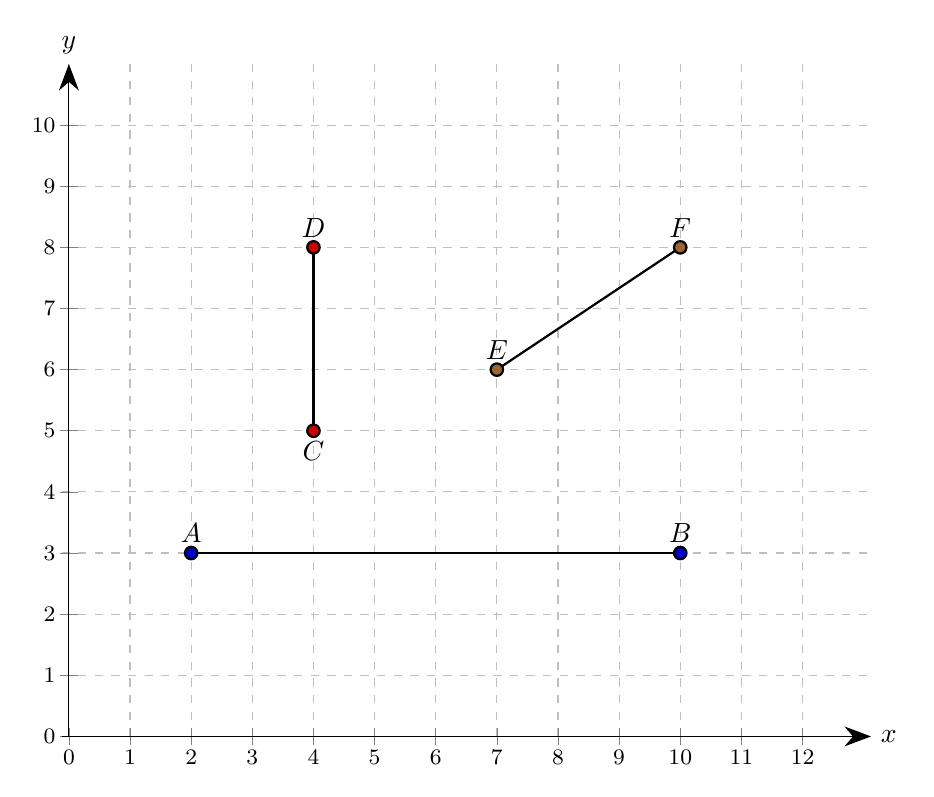
\begin{tikzpicture}[scale=1.5]
\begin{axis}[
    set layers,
    axis lines=middle,
    axis equal,
    %grid=both,
    grid, grid style=dashed,
    axis line style={-{Stealth[scale=2]}},
    xmax=11,
    ymax=11,
    xmin=2,
    ymin=0,
    xstep=1,
    ystep=1,
    xlabel=$x$, x label style={anchor=west}, 
    ylabel=$y$, y label style={anchor=south}, 
    ytick={0,...,10},
    xtick={0,...,12},
    extra y ticks={0},
    extra x ticks={0},
    ticklabel style={font=\footnotesize, fill=white, inner sep=1.5pt},
    mark size=1.5pt
    ]
\addplot+[color=black, thick=2,
      mark=*,
      ] coordinates{(2,3) (10,3)}
      node[pos=0,above] {$A$} node[pos=1,above] {$B$};
\addplot+[color=black, thick=2,
      mark=*,
      ] coordinates{(4,5) (4,8)}
      node[pos=0,below] {$C$} node[pos=1,above] {$D$};
\addplot+[color=black, thick=2,
      mark=*,
      ] coordinates{(7,6) (10,8)}
      node[pos=0,above] {$E$} node[pos=1,above] {$F$};
\end{axis}
\end{tikzpicture}
\end{minipage}
\begin{minipage}{0.3\textwidth}
    \(A(2;3)\)\\
    \(B(10;3)\)\\
    \(C(4;5)\)\\
    \(D(4;8)\)\\
    \(E(7;6)\)\\
    \(F(10;8)\)\\
\end{minipage}

\vspace{1cm}
Calcolo del segmento \(\overline{AB}\):
\[\overline{AB}=x_B-x_A\quad x_B>x_A\]
Calcolo del segmento \(\overline{CD}\):
\[\overline{CD}=y_D-y_C\quad y_D>y_C\]
Calcolo del segmento \(\overline{EG}\), si usa il Teorema di Pitagora:
\[\overline{EF}=\sqrt{(y_F-y_E)^2+(x_F-x_E)^2}\quad y_F>y_E \quad x_F>x_E\]


\clearpage
\textbf{Esercizio 1}: Ricopia sul quaderno il grafico cartesiano e indica le coordinate dei punti \(A\), \(B\) e \(C\). Poi calcola la lunghezza dei segmenti \(\overline{AB}\), \(\overline{BC}\) e \(\overline{AC}\).\\
\begin{minipage}{0.7\textwidth}
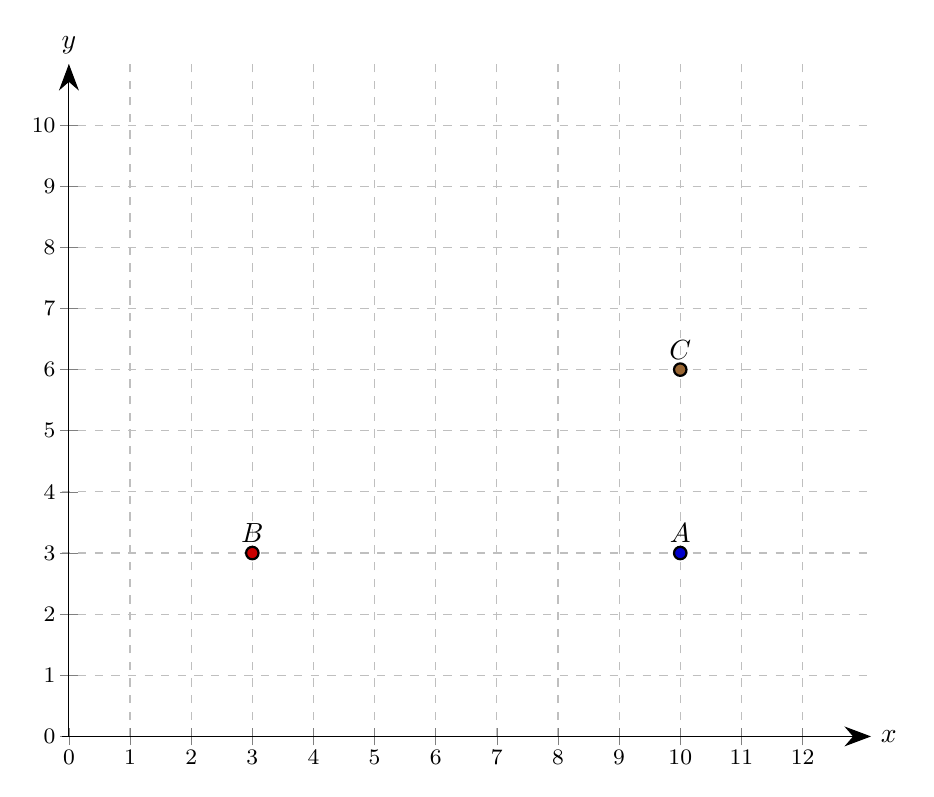
\begin{tikzpicture}[scale=1.5]
\begin{axis}[
    set layers,
    axis lines=middle,
    axis equal,
    %grid=both,
    grid, grid style=dashed,
    axis line style={-{Stealth[scale=2]}},
    xmax=11,
    ymax=11,
    xmin=2,
    ymin=0,
    xstep=1,
    ystep=1,
    xlabel=$x$, x label style={anchor=west}, 
    ylabel=$y$, y label style={anchor=south}, 
    ytick={0,...,10},
    xtick={0,...,12},
    extra y ticks={0},
    extra x ticks={0},
    ticklabel style={font=\footnotesize, fill=white, inner sep=1.5pt},
    mark size=1.5pt
    ]
\addplot+[color=black, thick=2,
      mark=*,
      ] coordinates{(10,3)}
      node[pos=0,above] {$A$};
\addplot+[color=black, thick=2,
      mark=*,
      ] coordinates{(3,3)}
      node[pos=0,above] {$B$};
\addplot+[color=black, thick=2,
      mark=*,
      ] coordinates{(10,6)}
      node[pos=0,above] {$C$};
\end{axis}
\end{tikzpicture}
\end{minipage}
\begin{minipage}{0.3\textwidth}
    \(A(?;?)\)\\
    \(B(?;?)\)\\
    \(C(?;?)\)\\
\end{minipage}
\vspace{1cm}

\textbf{Esercizio 2}: Ricopia sul quaderno il grafico cartesiano e indica le coordinate dei punti  \(A\), \(B\), \(C\) e \(D\) con le giuste coordinate. Poi calcola la lunghezza dei segmenti \(\overline{AB}\), \(\overline{BC}\), \(\overline{CD}\) e \(\overline{DA}\).\\
\begin{minipage}{0.7\textwidth}
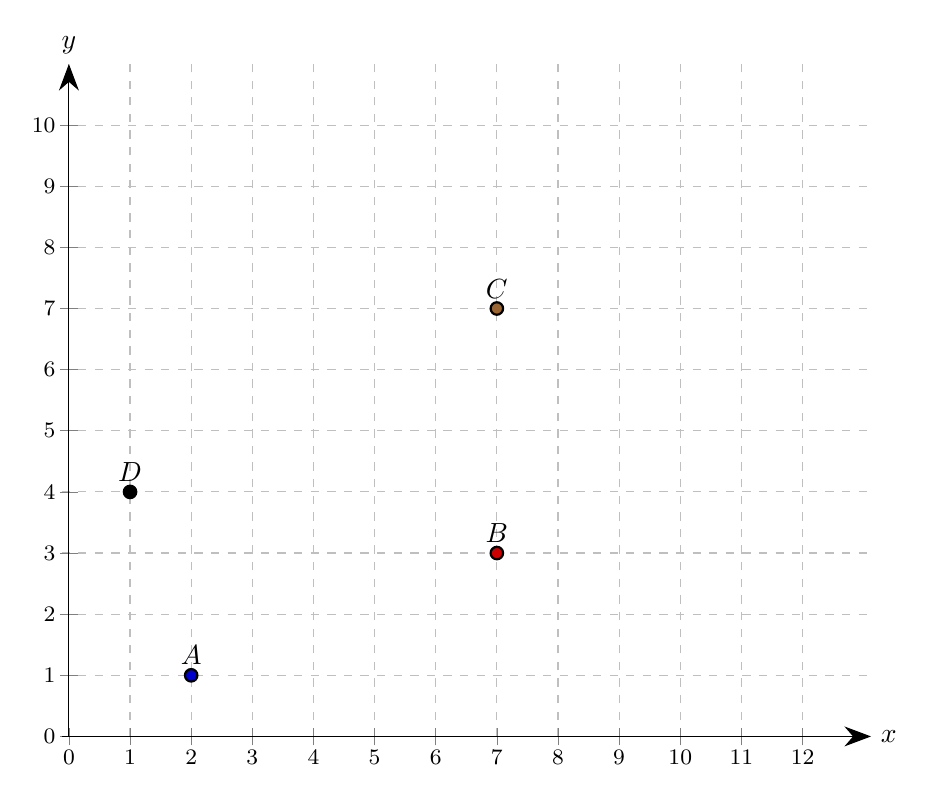
\begin{tikzpicture}[scale=1.5]
\begin{axis}[
    set layers,
    axis lines=middle,
    axis equal,
    %grid=both,
    grid, grid style=dashed,
    axis line style={-{Stealth[scale=2]}},
    xmax=11,
    ymax=11,
    xmin=2,
    ymin=0,
    xstep=1,
    ystep=1,
    xlabel=$x$, x label style={anchor=west}, 
    ylabel=$y$, y label style={anchor=south}, 
    ytick={0,...,10},
    xtick={0,...,12},
    extra y ticks={0},
    extra x ticks={0},
    ticklabel style={font=\footnotesize, fill=white, inner sep=1.5pt},
    mark size=1.5pt
    ]
\addplot+[color=black, thick=2,
      mark=*,
      ] coordinates{(2,1)}
      node[pos=0,above] {$A$};
\addplot+[color=black, thick=2,
      mark=*,
      ] coordinates{(7,3)}
      node[pos=0,above] {$B$};
\addplot+[color=black, thick=2,
      mark=*,
      ] coordinates{(7,7)}
      node[pos=0,above] {$C$};
\addplot+[color=black, thick=2,
      mark=*,
      ] coordinates{(1,4)}
      node[pos=0,above] {$D$};
\end{axis}
\end{tikzpicture}
\end{minipage}
\begin{minipage}{0.3\textwidth}
    \(A(?;?)\)\\
    \(B(?;?)\)\\
    \(C(?;?)\)\\
    \(D(?;?)\)\\
\end{minipage}
\vspace{1cm}

\textbf{Esercizio 3}: ricopia sul quaderno il grafico cartesiano, indica le coordinate dei punti \(A\), \(B\), \(C\) e \(D\). Calcola la lunghezza dei segmenti \(\overline{AB}\), \(\overline{BC}\), \(\overline{CD}\) e \(\overline{DA}\).\\
\begin{minipage}{0.7\textwidth}
\begin{tikzpicture}[scale=1.5]
\begin{axis}[
    set layers,
    axis lines=middle,
    axis equal,
    %grid=both,
    grid, grid style=dashed,
    axis line style={-{Stealth[scale=2]}},
    xmax=11,
    ymax=11,
    xmin=2,
    ymin=0,
    xstep=1,
    ystep=1,
    xlabel=$x$, x label style={anchor=west}, 
    ylabel=$y$, y label style={anchor=south}, 
    ytick={0,...,10},
    xtick={0,...,12},
    extra y ticks={0},
    extra x ticks={0},
    ticklabel style={font=\footnotesize, fill=white, inner sep=1.5pt},
    mark size=1.5pt
    ]
% \addplot+[color=black, thick=2,
%       mark=*,
%       ] coordinates{(10,3)}
%       node[pos=0,above] {$A$};
% \addplot+[color=black, thick=2,
%       mark=*,
%       ] coordinates{(3,3)}
%       node[pos=0,above] {$B$};
% \addplot+[color=black, thick=2,
%       mark=*,
%       ] coordinates{(10,6)}
%       node[pos=0,above] {$C$};
% \addplot+[color=black, thick=2,
%       mark=*,
%       ] coordinates{(3,6)}
%       node[pos=0,above] {$D$};
\end{axis}
\end{tikzpicture}
\end{minipage}
\begin{minipage}{0.3\textwidth}
    \(A(10;3)\)\\
    \(B(3;3)\)\\
    \(C(3;6)\)\\
    \(D(10;6)\)\\
\end{minipage}
\vspace{1cm}

\textbf{Esercizio 4}: ricopia sul quaderno il grafico cartesiano, indica le coordinate dei punti \(A\), \(B\), \(C\) e \(D\). Calcola la lunghezza dei segmenti \(\overline{AB}\), \(\overline{BC}\), \(\overline{CD}\) e \(\overline{DA}\). \\
\begin{minipage}{0.7\textwidth}
\begin{tikzpicture}[scale=1.5]
\begin{axis}[
    set layers,
    axis lines=middle,
    axis equal,
    %grid=both,
    grid, grid style=dashed,
    axis line style={-{Stealth[scale=2]}},
    xmax=11,
    ymax=11,
    xmin=2,
    ymin=0,
    xstep=1,
    ystep=1,
    xlabel=$x$, x label style={anchor=west}, 
    ylabel=$y$, y label style={anchor=south}, 
    ytick={0,...,10},
    xtick={0,...,12},
    extra y ticks={0},
    extra x ticks={0},
    ticklabel style={font=\footnotesize, fill=white, inner sep=1.5pt},
    mark size=1.5pt
    ]
% \addplot+[color=black, thick=2,
%       mark=*,
%       ] coordinates{(11,2)}
%       node[pos=0,above] {$A$};
% \addplot+[color=black, thick=2,
%       mark=*,
%       ] coordinates{(4,2)}
%       node[pos=0,above] {$B$};
% \addplot+[color=black, thick=2,
%       mark=*,
%       ] coordinates{(11,5)}
%       node[pos=0,above] {$D$};
% \addplot+[color=black, thick=2,
%       mark=*,
%       ] coordinates{(4,7)}
%       node[pos=0,above] {$C$};
\end{axis}
\end{tikzpicture}
\end{minipage}
\begin{minipage}{0.3\textwidth}
    \(A(11;2)\)\\
    \(B(4;2)\)\\
    \(C(4;7)\)\\
    \(D(11;5)\)\\
\end{minipage}
\end{document}